\chapter{जीवाणु-विज्ञान: वृद्धि, शरीरक्रिया और आनुवंशिकी}\label{ch:b3:bacteriology}

गर्म शोरबे में \emph{Escherichia coli} की कोई एक कोशिका हर बीस मिनट में
विभाजित होती है। बिना रोक-टोक उसके वंशज दो दिन में पृथ्वी से भारी हो
जाते; असल में वे घंटों में रुक जाते हैं, जब शर्करा चुक जाती है, और
हफ़्तों तक ऐसी अवस्था में बैठे रहते हैं जो भुखमरी झेल जाती है। कोई
संबंधी जीवाणु, किसी घाव और कुछ घंटों के साथ, दस करोड़ कोशिकाएँ और कोई
ज्वर बन जाता है; सौ वर्ष पहले वह अपने संक्रमित रोगियों में से
एक-तिहाई को मार देता था, और 1941 से उसके विरुद्ध किसी फफूँद के विष ने
किसी भी दूसरी औषध से अधिक जान बचाई है --- जबकि जीवाणुओं ने उन्हीं अस्सी
वर्षों में हर बने \omterm{def:b3:bacteriology:antibiotics}{प्रतिजैविक} से बचने के रास्ते विकसित कर लिए हैं।
जीवाणु वही जीव हैं जिनमें पहली बार दिखाया गया कि जीन DNA हैं, जिनमें
जीन-नियमन पहली बार समझा गया, और जिनसे
\cref{ch:b3:genetic-engineering} के औज़ार लिए गए। यह अध्याय उन्हें जीव
के रूप में लेता है: उनका आवरण, किसी फ्लास्क में और किसी सतत संवर्धन में
उनकी वृद्धि का अंकगणित, कोई समष्टि अपना घनत्व कैसे भाँपती है,
कोशिकाओं के बीच जीनों का यातायात, और \omterm{def:b3:bacteriology:antibiotics}{प्रतिजैविकों} तथा प्रतिरोध की रसायन
और विकास-कथा।

\section{जीवाणु कोशिका}

\begin{definition}[आवरण]\label{def:b3:bacteriology:envelope}
\index{पेप्टिडोग्लाइकन}\index{ग्राम-धनात्मक}\index{ग्राम-ऋणात्मक}\index{बाह्य झिल्ली}\index{लिपोपॉलिसैकेराइड}\index{अंतःबीजाणु}
थोड़े-से को छोड़कर हर जीवाणु \emph{पेप्टिडोग्लाइकन} की दीवार में बंद है:
बारी-बारी से N-ऐसीटिलग्लूकोसैमीन और N-ऐसीटिलम्यूरैमिक अम्ल की शृंखलाएँ,
जो छोटे पेप्टाइडों से तिर्यक-बद्ध होकर एक ही अणु बन जाती हैं और कोशिका
को घेरकर कोशिकाद्रव्य के स्फीति-दाब --- कई वायुमंडल --- का प्रतिरोध
करती हैं। \emph{ग्राम-धनात्मक} जीवाणुओं की दीवार मोटी होती है,
\qtyrange{20}{80}{nm} की, कई परतों वाली, और उसमें टाइकोइक अम्ल पिरोए
रहते हैं; \emph{ग्राम-ऋणात्मक} जीवाणुओं की दीवार एक-दो परतों की पतली
होती है और उसके बाहर एक दूसरी लिपिड द्विपरत, यानी \emph{बाह्य झिल्ली},
जिसका बाहरी पटल \emph{लिपोपॉलिसैकेराइड} (LPS, अंतर्विष --- वही अणु
जिसे \cref{ch:b3:innate-immunity} का जन्मजात प्रतिरक्षा-तंत्र पहचानता
है और जो पूतिज आघात करता है) है और जो किसी परिकोशिकाद्रव्य को घेरे रहती
है। बाह्य झिल्ली के पोरिन छोटे अणुओं को आने देते हैं और अनेक
\omterm{def:b3:bacteriology:antibiotics}{प्रतिजैविकों} को रोक देते हैं। बाहर भक्षकाणुओं के विरुद्ध कोई
पॉलिसैकेराइड संपुट, तैरने के लिए कशाभ
(\cref{ch:b3:cytoskeleton-motility}) और जुड़ाव तथा
\omterm{def:b3:bacteriology:hgt}{संयुग्मन} के लिए पिली हो सकते हैं। भीतर गुणसूत्र --- अधिकांश जातियों में
\qtyrange{1}{10}{Mb} का एक ही वलयाकार अणु --- बिना किसी झिल्ली के किसी
केंद्रकाभ में मुड़ा रहता है, और साथ में \omterm{def:b3:genetic-engineering:tools}{प्लाज़्मिड}। कुछ वंश
(\emph{Bacillus}, \emph{Clostridium}) गुणसूत्र की एक प्रति को किसी मोटे
आवरण में \emph{अंतःबीजाणु} के रूप में बंद कर सकते हैं, जो निर्जलित और
उपापचय की दृष्टि से निष्क्रिय होता है, उबलना, विकिरण और सदियों का सूखा
झेल जाता है, और पोषक लौटने पर अंकुरित होता है।
\end{definition}

\begin{method}[ग्राम अभिरंजन]\label{met:b3:bacteriology:gram}
\index{ग्राम अभिरंजन}
जीवाणु-विज्ञान की प्रयोगशाला का सबसे पुराना परीक्षण (ग्राम, 1884) आज भी
\omterm{def:b3:bacteriology:antibiotics}{प्रतिजैविक} का पहला चुनाव तय करता है। (1) प्रतिदर्श को फैलाकर ताप से
स्थिर कीजिए; (2) क्रिस्टल वायलेट से, फिर आयोडीन से अभिरंजित कीजिए, जो
कोशिकाओं के भीतर रंजक के साथ कोई बड़ा अविलेय संकुल बनाता है; (3) ऐल्कोहल
से धोइए: \omterm{def:b3:bacteriology:envelope}{ग्राम-धनात्मकों} की मोटी \omterm{def:b3:bacteriology:envelope}{पेप्टिडोग्लाइकन}, जो ऐल्कोहल से
निर्जलित हो जाती है, संकुल को फँसा लेती है और कोशिकाएँ बैंगनी रहती हैं,
जबकि \omterm{def:b3:bacteriology:envelope}{ग्राम-ऋणात्मकों} की पतली दीवार उसे बाहर जाने देती है; (4) सफ़्रानिन
से प्रति-अभिरंजन कीजिए, जो अब रंगहीन हुए \omterm{def:b3:bacteriology:envelope}{ग्राम-ऋणात्मकों} को गुलाबी कर
देता है। आकार और विन्यास --- गुच्छों में गोलाणु (स्टैफ़िलोकोकस) या
शृंखलाओं में (स्ट्रेप्टोकोकस), दंडाणु, कुंडलाणु --- पहचान और सँकरी कर
देते हैं, और किसी फोड़े से मिला गुच्छों वाला बैंगनी गोलाणु किसी
संवर्धन के उगने से पहले ही स्टैफ़िलोकोकस है।
\end{method}

\begin{omfigure}
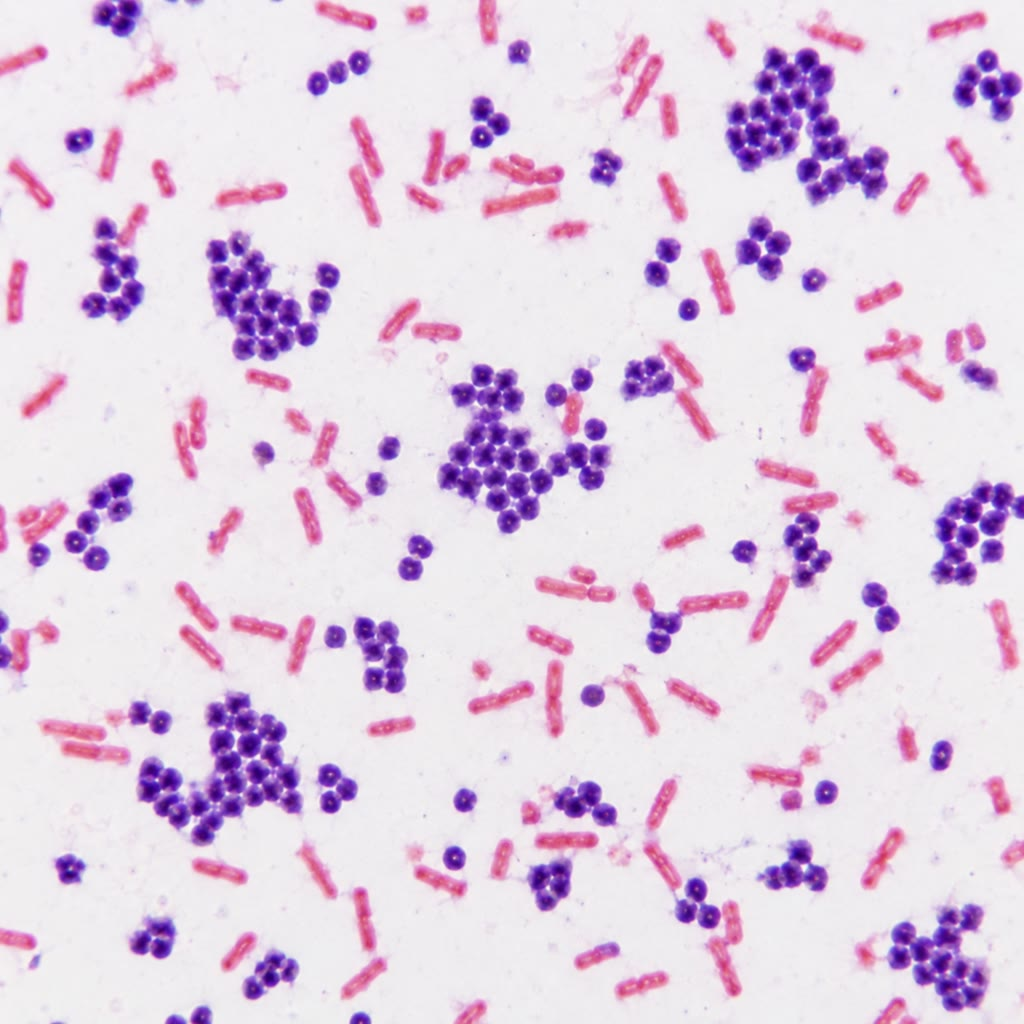
\includegraphics[width=0.36\linewidth]{images/book5/ai/b5-12-gram-stain.jpg}\hspace{0.04\linewidth}
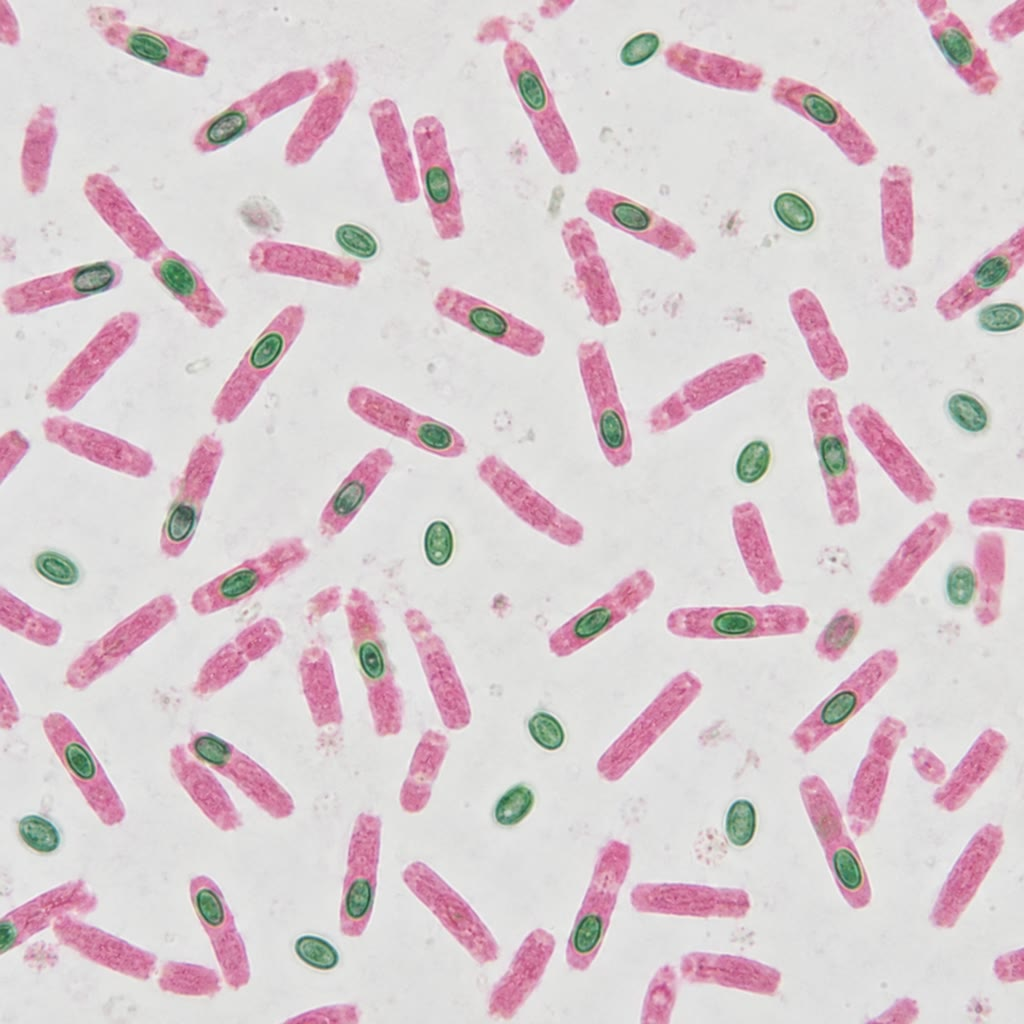
\includegraphics[width=0.36\linewidth]{images/book5/ai/b5-12-endospores.jpg}

{\small बाएँ: कोई \omterm{met:b3:bacteriology:gram}{ग्राम अभिरंजन} --- गुच्छों में बैंगनी \omterm{def:b3:bacteriology:envelope}{ग्राम-धनात्मक}
गोलाणु, गुलाबी \omterm{def:b3:bacteriology:envelope}{ग्राम-ऋणात्मक} दंडाणु। दाएँ: \omterm{def:b3:bacteriology:envelope}{अंतःबीजाणुओं} के लिए
अभिरंजित \emph{Bacillus} कोशिकाएँ, जिनमें गुलाबी कोशिकाओं के भीतर चमकीले
हरे अंडाकार और उनके बगल में मुक्त बीजाणु हैं।}
\end{omfigure}

\begin{omfigure}
\begin{tikzpicture}[every node/.style={font=\scriptsize}, >=stealth]
  % Gram-positive
  \begin{scope}
    \fill[omDef!15] (0,0) rectangle (4.5,0.4); \draw[thick, omDef] (0,0) -- (4.5,0); \draw[thick, omDef] (0,0.4) -- (4.5,0.4);
    \fill[omProp!40] (0,0.5) rectangle (4.5,2.0); \foreach \y in {0.7,0.95,1.2,1.45,1.7} \draw[omProp!80!black, thin] (0,\y) -- (4.5,\y);
    \foreach \x in {0.6,1.6,2.6,3.6} \draw[omMeth!70!black, thick] (\x,0.5) -- (\x,2.3);
    \node[below] at (2.25,-0.1) {कोशिकाद्रव्यी झिल्ली};
    \node[right, align=left] at (4.6,1.25) {मोटी पेप्टिडोग्लाइकन\\(\qtyrange{20}{80}{nm})}; \node[right, omMeth!70!black] at (4.6,2.2) {टाइकोइक अम्ल};
    \node[above, font=\small\bfseries] at (2.25,2.5) {ग्राम-धनात्मक};
  \end{scope}
  % Gram-negative
  \begin{scope}[xshift=8.6cm]
    \fill[omDef!15] (0,0) rectangle (4.5,0.4); \draw[thick, omDef] (0,0) -- (4.5,0); \draw[thick, omDef] (0,0.4) -- (4.5,0.4);
    \fill[omProp!40] (0,0.75) rectangle (4.5,1.05); \draw[omProp!80!black, thin] (0,0.9) -- (4.5,0.9);
    \fill[omDef!15] (0,1.5) rectangle (4.5,1.9); \draw[thick, omDef] (0,1.5) -- (4.5,1.5); \draw[thick, omDef] (0,1.9) -- (4.5,1.9);
    \foreach \x in {0.4,0.9,1.4,1.9,2.4,2.9,3.4,3.9} \draw[omThm, thick] (\x,1.9) -- (\x,2.35);
    \draw[thick, fill=white] (2.0,1.45) rectangle (2.5,1.95); \node[below, font=\tiny] at (2.25,1.45) {पोरिन};
    \node[below] at (2.25,-0.1) {कोशिकाद्रव्यी झिल्ली};
    \node[right] at (4.6,0.9) {पतली पेप्टिडोग्लाइकन}; \node[right] at (4.6,1.7) {बाह्य झिल्ली}; \node[right, omThm] at (4.6,2.25) {LPS (अंतर्विष)};
    \node[right, font=\tiny] at (4.6,1.27) {परिकोशिकाद्रव्य};
    \node[above, font=\small\bfseries] at (2.25,2.5) {ग्राम-ऋणात्मक};
  \end{scope}
\end{tikzpicture}

{\small दोनों आवरण। \omterm{def:b3:bacteriology:envelope}{ग्राम-धनात्मक} झिल्ली को \omterm{def:b3:bacteriology:envelope}{पेप्टिडोग्लाइकन} की अनेक
परतों में लपेटते हैं; \omterm{def:b3:bacteriology:envelope}{ग्राम-ऋणात्मकों} की परत पतली है और उनके पास
\omterm{def:b3:bacteriology:envelope}{लिपोपॉलिसैकेराइड} की कोई \omterm{def:b3:bacteriology:envelope}{बाह्य झिल्ली} है जिसमें पोरिन छिदे हैं, और वही
अनेक \omterm{def:b3:bacteriology:antibiotics}{प्रतिजैविकों} को बाहर रखती है तथा वह अंतर्विष बनाती है जो पूतिज
आघात करता है।}
\end{omfigure}

\section{वृद्धि}

\begin{theorem}[चरघातांकी वृद्धि, मोनो नियम और केमोस्टैट]\label{thm:b3:bacteriology:monod}
\index{चरघातांकी वृद्धि!जीवाणु}\index{मोनो समीकरण}\index{केमोस्टैट}\index{तनुकरण दर}
$N$ कोशिकाओं की कोई समष्टि, जो पीढ़ी-काल $T$ से विभाजित होती है,
$N(t) = N_{0}\,2^{t/T} = N_{0}e^{\mu t}$ की तरह बढ़ती है, जिसमें विशिष्ट
वृद्धि दर $\mu =
\ln 2/T$ है। यह दर सीमांतकारी पोषक $S$ पर
\emph{मोनो नियम} से निर्भर करती है
\[
\mu(S) = \mu_{\max}\,\frac{S}{K_{S} + S},
\]
जो $\mu_{\max}$ पर संतृप्त होता है और $S = K_{S}$ पर अर्ध-अधिकतम होता
है। किसी \emph{केमोस्टैट} में --- आयतन $V$ का कोई पात्र जिसमें पोषक
सांद्रता $S_{0}$ का ताज़ा माध्यम दर $F$ से बहता है और जिससे संवर्धन उसी
दर से निकलता है, और \omterm{thm:b3:bacteriology:monod}{तनुकरण दर} $D = F/V$ है --- स्थायी अवस्था में
\[
\mu(S^{*}) = D,\qquad S^{*} = \frac{K_{S}D}{\mu_{\max} - D},\qquad
X^{*} = Y\,(S_{0} - S^{*}),
\]
होता है, जहाँ $X$ कोशिका-घनत्व है और $Y$ उपज (प्रति इकाई पोषक बनी
कोशिकाएँ)। प्रयोगकर्ता कोई पंप घुमाकर वृद्धि दर तय करता है; संवर्धन
अपने पीछे छोड़े पोषक को समायोजित करके अनुक्रिया देता है। यदि $D$
$\mu(S_{0})$ से अधिक हो तो कोशिकाएँ साथ नहीं दे पातीं और बह जाती हैं।
\end{theorem}
\begin{proof}
कोशिकाएँ: $\mathrm{d}X/\mathrm{d}t = \mu(S)X - DX$, यानी वृद्धि घटा
बहिर्गम; $X^{*} > 0$ के साथ स्थायी अवस्था पर $\mu(S^{*}) = D$, और मोनो
नियम को उलटने से $S^{*}$ मिलता है। पोषक: $\mathrm{d}S/\mathrm{d}t = D(S_{0} -
S) - \mu(S)X/Y$, यानी अंतर्गम घटा बहिर्गम घटा खपत; स्थायी
अवस्था पर, $\mu = D$ के साथ, $D(S_{0} - S^{*}) = DX^{*}/Y$, जिससे $X^{*}$
मिलता है। स्थायी अवस्था तभी होती है जब $S^{*} < S_{0}$ हो, यानी $D <
\mu(S_{0})$; उससे आगे एकमात्र स्थायी अवस्था $X = 0$ है, यानी बह जाना।
स्थायित्व: यदि $X$ $X^{*}$ से ऊपर उठे तो वह अधिक खपाता है, $S$
$S^{*}$ से नीचे गिरता है, $\mu$ $D$ से नीचे गिरता है और $X$ घट जाता है
--- पोषक के ज़रिए एक ऋण पुनर्भरण।
\end{proof}

\begin{example}[संख्याओं में कोई संवर्धन]\label{ex:b3:bacteriology:numbers}
\qty{37}{\celsius} पर समृद्ध माध्यम में \emph{E.~coli}: $T = \qty{20}{min}$,
$\mu = \qty{2.1}{h^{-1}}$। एक कोशिका से बारह घंटे बाद $2^{36}$
--- $7\times 10^{10}$ कोशिकाएँ, यानी लगभग \qty{70}{mg}, और यहीं कोई
\qty{100}{mL} फ्लास्क ऑक्सीजन तथा शर्करा के अभाव में रुक जाता है; ``दो
दिन में पृथ्वी का द्रव्यमान'' $2^{144}\approx 10^{43}$ कोशिकाएँ हैं, और
अंकगणित केवल यह दिखाता है कि चरघातांकी वृद्धि कभी टिकती नहीं। ग्लूकोज़
पर किसी केमोस्टैट में $\mu_{\max} = \qty{1.0}{h^{-1}}$, $K_{S} =
\qty{0.01}{g/L}$, $S_{0} = \qty{1}{g/L}$ और $Y = \qty{0.5}{g}$
कोशिकाएँ प्रति ग्राम ग्लूकोज़ के साथ, \qty{0.5}{h^{-1}} की \omterm{thm:b3:bacteriology:monod}{तनुकरण दर}
पर ग्लूकोज़ $S^{*}
= 0.01\times 0.5/0.5 = \qty{0.01}{g/L}$ बचता है और कोशिकाएँ $X^{*} =
\qty{0.495}{g/L}$ पर रहती हैं, हर \qty{83}{min} में विभाजित होती हुईं,
अनिश्चित काल तक। किसी नियत वृद्धि दर की शरीरक्रिया केमोस्टैट से ही
पढ़ी जाती है, और हज़ारों पीढ़ियों का विकास किसी बोतल में इसी से चलाया
जाता है।
\end{example}

\begin{omfigure}
\begin{tikzpicture}
\begin{axis}[
  width=6.6cm, height=5.4cm,
  axis x line=bottom, axis y line=left,
  xmin=0, xmax=14, ymin=1e6, ymax=1e10, ymode=log,
  xlabel={घंटे}, ylabel={प्रति mL कोशिकाएँ},
  xlabel style={font=\small, at={(axis description cs:0.5,-0.12)}, anchor=north}, ylabel style={font=\small},
  tick label style={font=\scriptsize}, xtick={0,4,8,12},
  clip=false,
]
\addplot[very thick, omDef, domain=0:1.5, samples=2] {1e6};
\addplot[very thick, omDef, domain=1.5:7.5, samples=40] {1e6*2^((x-1.5)/0.5)};
\addplot[very thick, omDef, domain=7.5:12, samples=2] {4.1e9};
\addplot[very thick, omDef, domain=12:14, samples=10] {4.1e9*exp(-0.15*(x-12))};
\node[font=\scriptsize, anchor=south] at (axis cs:0.8,1.2e6) {विलंब};
\node[font=\scriptsize, anchor=west] at (axis cs:2.5,3e8) {चरघातांकी: $T = \qty{30}{min}$};
\node[font=\scriptsize, anchor=north] at (axis cs:10,3.5e9) {स्थिर};
\node[font=\scriptsize, anchor=north] at (axis cs:12.8,2.2e9) {मृत्यु};
\end{axis}
\begin{axis}[
  at={(7.8cm,0)}, anchor=south west,
  width=6.6cm, height=5.4cm,
  axis x line=bottom, axis y line=left,
  xmin=0, xmax=0.1, ymin=0, ymax=1.1,
  xlabel={ग्लूकोज़ $S$ (g/L)}, ylabel={$\mu$ (h$^{-1}$)},
  xlabel style={font=\small, at={(axis description cs:0.5,-0.12)}, anchor=north}, ylabel style={font=\small},
  tick label style={font=\scriptsize}, xtick={0,0.01,0.05,0.1}, xticklabels={0,$K_S$,0.05,0.1}, ytick={0,0.5,1},
  clip=false,
]
\addplot[very thick, omThm, domain=0:0.1, samples=60] {x/(0.01+x)};
\addplot[dashed, gray, domain=0:0.1, samples=2] {1};
\addplot[dashed, gray] coordinates {(0.01,0) (0.01,0.5)}; \addplot[dashed, gray] coordinates {(0,0.5) (0.01,0.5)};
\node[font=\scriptsize, omThm, anchor=north west] at (axis cs:0.045,0.6) {मोनो: $\mu = \mu_{\max}S/(K_{S}+S)$};
\node[font=\scriptsize, gray, anchor=south east] at (axis cs:0.1,1.01) {$\mu_{\max}$};
\end{axis}
\end{tikzpicture}

{\small बाएँ: कोई बैच संवर्धन --- एंज़ाइमों के प्रेरित होते समय एक
विलंब, चरघातांकी वृद्धि, पोषक चुक जाने पर कोई \omterm{def:b3:bacteriology:phases}{स्थिर प्रावस्था}, और
धीमी मृत्यु। दाएँ: मोनो नियम, यानी सीमांतकारी पोषक के सामने वृद्धि दर,
जिसमें $K_{S}$ अर्ध-अधिकतम वृद्धि की सांद्रता है।}
\end{omfigure}

\begin{definition}[प्रावस्थाएँ और अवस्थाएँ]\label{def:b3:bacteriology:phases}
\index{विलंब प्रावस्था}\index{स्थिर प्रावस्था}\index{बीजाणुजनन}\index{सिग्मा कारक}
किसी ताज़ा फ्लास्क में (किसी \emph{बैच संवर्धन} में) कोशिकाएँ पहले रुकती
हैं --- यह \emph{विलंब प्रावस्था} है, जब वे नए माध्यम के लिए ज़रूरी
एंज़ाइम प्रेरित करती हैं --- फिर चरघातांकी रूप से बढ़ती हैं, फिर तब रुक
जाती हैं जब कोई पोषक चुक जाए या कोई अपशिष्ट जमा हो जाए: यही
\emph{स्थिर प्रावस्था} है, जिसमें कोशिकाएँ सिकुड़ती हैं, अपना आवरण मोटा
करती हैं, अपने केंद्रकाभ को रक्षक प्रोटीनों के चारों ओर संघनित करती
हैं, वैकल्पिक सिग्मा कारक RpoS के ज़रिए तनाव-जीन चालू करती हैं, और
महीनों जीवित रह सकती हैं; उसके बाद कोई मृत्यु प्रावस्था आती है जिसमें
अधिकांश कोशिकाएँ लयित हो जाती हैं और थोड़ी अवशेषों पर जीती रहती हैं।
कुछ जातियाँ भुखमरी का उत्तर किसी परिवर्धनी कार्यक्रम से देती हैं:
\emph{Bacillus subtilis} असममित रूप से विभाजित होता है और बड़ी कोशिका
छोटी को निगल लेती है और उसके चारों ओर बीजाणु बना देती है, यानी आठ
घंटों का ऐसा अनुक्रम जिसे \emph{सिग्मा कारकों} का एक प्रपात नियंत्रित
करता है --- वे उपइकाइयाँ जो RNA पॉलीमरेज़ को प्रवर्तकों के किसी एक
समुच्चय की ओर भेजती हैं --- और जो दोनों कक्षों के बीच बारी-बारी चलता है:
यह विभेदन का और दीवार के पार कोशिका-से-कोशिका संकेतन का पहला जीवाणु उदाहरण है।
\end{definition}

\section{एक-दूसरे को भाँपना}

\begin{definition}[गणपूर्ति संवेदन]\label{def:b3:bacteriology:quorum}
\index{गणपूर्ति संवेदन}\index{स्वप्रेरक}\index{द्वि-घटक तंत्र}
जीवाणु अपना घनत्व \emph{गणपूर्ति संवेदन} से पकड़ते हैं: हर कोशिका कोई
छोटा संकेत-अणु, यानी कोई \emph{स्वप्रेरक} --- \omterm{def:b3:bacteriology:envelope}{ग्राम-ऋणात्मकों} में
ऐसिलित होमोसेरीन लैक्टोन, \omterm{def:b3:bacteriology:envelope}{ग्राम-धनात्मकों} में छोटे पेप्टाइड ---
अचर दर से स्रावित करती है; माध्यम में सांद्रता कोशिकाओं की संख्या के
साथ चढ़ती है, और जब वह किसी देहली को पार करती है तो किसी ऐसे ग्राही से
बँध जाती है जो जीनों का एक समुच्चय चालू कर देता है, जिनमें स्वयं
स्वप्रेरक की सिंथेज़ भी है (इसीलिए यह नाम)। जिन जीनों पर यह नियंत्रण है
वे वही हैं जो केवल संगत में लाभ देते हैं: \emph{Vibrio fischeri} में
प्रकाश, \emph{Staphylococcus aureus} और \emph{Pseudomonas aeruginosa}
में विषालुता-कारक, जैवफ़िल्म की आधात्री, DNA ग्रहण के लिए सक्षमता, और
पड़ोसियों की हत्या। अधिकांश जीवाणु संवेदन
\emph{द्वि-घटक तंत्रों} से चलता है: कोई झिल्ली-स्थित हिस्टिडीन काइनेज़
जो किसी उद्दीपन को पकड़ती है और किसी कोशिकाद्रव्यी अनुक्रिया-नियामक का
फ़ॉस्फ़ोरिलन करती है, जो DNA से बँधता है --- किसी कोशिका के पास दर्जनों
हैं, फ़ॉस्फ़ेट, परासरणिता, ऑक्सीजन और दूसरी जातियों के स्वप्रेरकों के लिए।
\end{definition}

\begin{proof}[प्रमाण-सामग्री]
नीलसन, प्लैट और हेस्टिंग्स (1970) ने ज्योतिर्मय सामुद्रिक जीवाणु
\emph{Vibrio fischeri} को किसी तनु टीके से उगाया और पाया कि कोशिकाओं ने
तब तक कोई प्रकाश नहीं बनाया जब तक वे प्रति मिलीलीटर कोई $10^{7}$ के
घनत्व तक न पहुँच गईं, और फिर सब एक साथ जल उठीं; जिस माध्यम में कोई सघन
संवर्धन उगा हो उसे निर्जर्मित करके किसी तनु संवर्धन में जोड़ने पर
प्रकाश तुरंत चालू हो गया। कोशिकाएँ किसी स्रावित पदार्थ को गिन रही
थीं, समय या पोषक को नहीं। वह पदार्थ कोई ऐसिल-होमोसेरीन लैक्टोन पहचाना
गया (एबरहार्ड, 1981), और जीन --- सिंथेज़ के लिए \emph{luxI},
ग्राही के लिए \emph{luxR}, और जिस ल्यूसिफ़रेज़ प्रकार्यगुच्छ पर उनका
नियंत्रण है --- \emph{E.~coli} में क्लोनित किए गए, जो तब भीड़ में चमकने
लगा। जो स्क्विड इस जीवाणु को प्रति मिलीलीटर $10^{10}$ पर बसाता है उसका
प्रकाश-अंग चमकता है; समुद्र में, जहाँ जीवाणु तनु हैं, वे अँधेरे रहते
हैं और लागत बचा लेते हैं।
\end{proof}

\begin{proposition}[घनत्व की एक देहली]\label{prop:b3:bacteriology:threshold}
\index{गणपूर्ति संवेदन!देहली}
मान लीजिए $N$ कोशिकाओं में से, जो आयतन $V$ में हैं, हर एक \omterm{def:b3:bacteriology:quorum}{स्वप्रेरक} को प्रति
सेकंड $p$ अणुओं की दर से स्रावित करती है, और अणु प्रथम-कोटि दर
$k$ से खोता है (अपघटित या तनु होकर)। सांद्रता
$A^{*} = pN/(kV)$ की ओर जाती है, जो कोशिका-घनत्व $N/V$ के समानुपाती है,
और काल-नियतांक $1/k$ है; ग्राही तब चालू होता है जब $A^{*}$ अपनी देहली
$A_{\text{देहली}}$ तक पहुँचे, यानी इस घनत्व पर
\[
\left(\frac{N}{V}\right)_{\text{देहली}} = \frac{k\,A_{\text{देहली}}}{p}.
\]
किसी बंद स्थान में --- किसी स्क्विड के प्रकाश-अंग, किसी फोड़े, किसी
फेफड़े के श्लेष्म में --- $k$ छोटा होता है क्योंकि संकेत बहकर नहीं जाता,
इसलिए देहली-घनत्व कम कोशिकाओं से ही आ जाता है; खुले पानी में वह कभी
नहीं आता। इसलिए कोशिका अपनी संख्या नहीं, बल्कि उस आयतन की प्रति इकाई
अपनी संख्या मापती है जिसे वह साझा करती है, और किसी भी सहकारी कार्य के
लिए यही मायने रखता है; और \omterm{def:b3:bacteriology:quorum}{स्वप्रेरक} का अपनी ही सिंथेज़ पर धन पुनर्भरण
स्विच को तीखा बना देता है: एक बार थोड़ी कोशिकाएँ देहली पार कर लें, तो
उनका अतिरिक्त उत्पादन बाकी को भी पार करा देता है।
\end{proposition}
\begin{proof}
$\mathrm{d}A/\mathrm{d}t = pN/V - kA$ की स्थायी अवस्था $A^{*} =
pN/(kV)$ है और वह उस तक $e^{-kt}$ की तरह पहुँचता है। $A^{*} = A_{\text{देहली}}$
रखकर $N/V$ के लिए हल करने पर देहली-घनत्व मिलता है।
\end{proof}

\begin{omfigure}
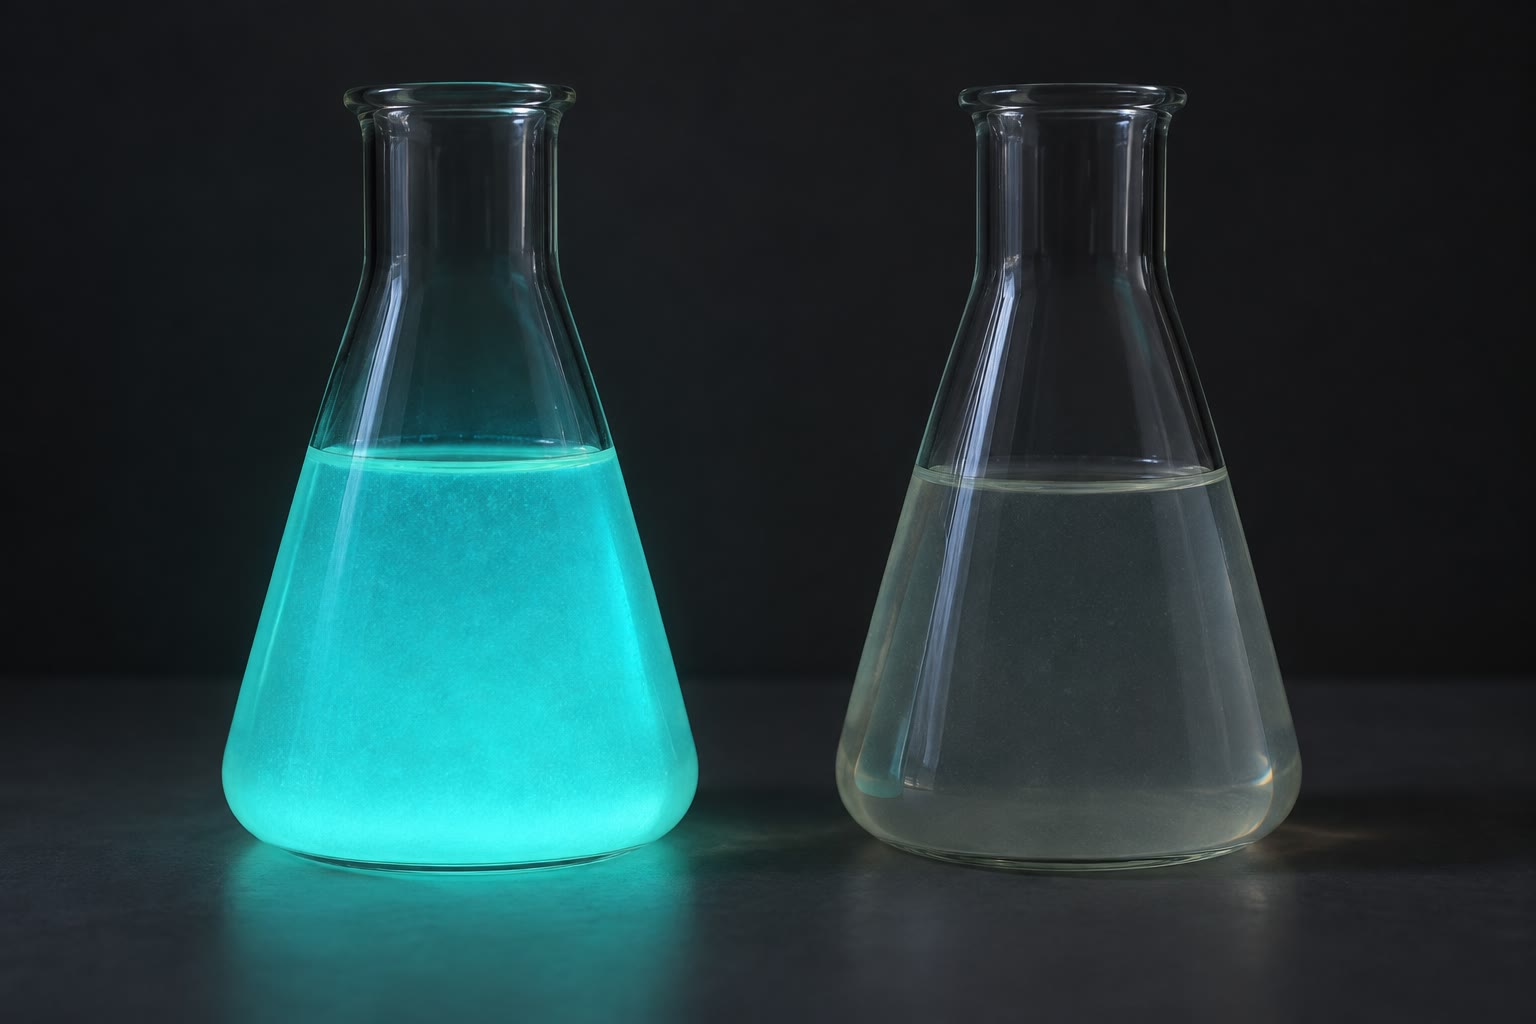
\includegraphics[width=0.46\linewidth]{images/book5/ai/b5-12-quorum-glow.jpg}\hspace{0.04\linewidth}
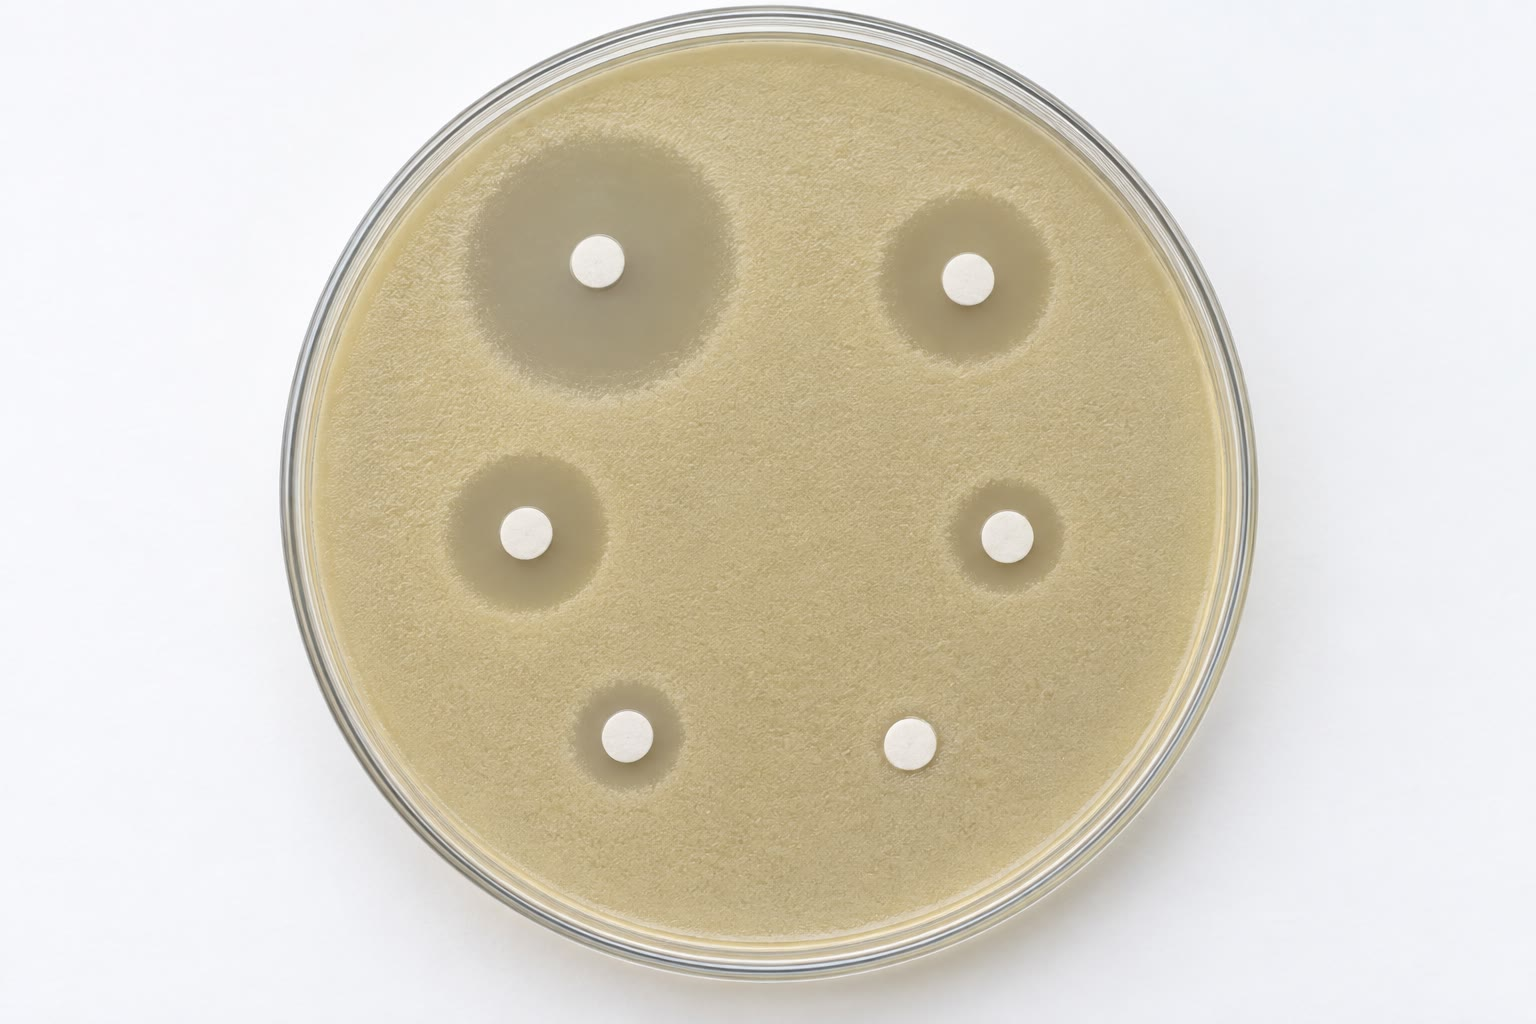
\includegraphics[width=0.46\linewidth]{images/book5/ai/b5-12-antibiotic-disks.jpg}

{\small बाएँ: \emph{Vibrio fischeri} का कोई सघन संवर्धन चमकता हुआ, उसके
बगल में कोई तनु संवर्धन जो अँधेरा है --- वही कोशिकाएँ, अपनी गणपूर्ति के
ऊपर और नीचे। दाएँ: कोई \omterm{met:b3:bacteriology:mic}{चक्रिका-विसरण} परीक्षण; हर स्वच्छ क्षेत्र का
व्यास उस चक्रिका पर रखे \omterm{def:b3:bacteriology:antibiotics}{प्रतिजैविक} के प्रति जीवाणु की संवेदिता मापता
है, और जिस चक्रिका के चारों ओर कोई क्षेत्र न हो वह किसी प्रतिरोध को
चिह्नित करती है।}
\end{omfigure}

\section{जीनों का यातायात}

\begin{definition}[क्षैतिज जीन-स्थानांतरण]\label{def:b3:bacteriology:hgt}
\index{रूपांतरण}\index{संचारण}\index{संयुग्मन}\index{प्लाज़्मिड!प्रतिरोध}\index{चल आनुवंशिक अवयव}\index{समग्र जीनोम}
जीवाणु क्लोनी रूप से जनन करते हैं पर जीनों का विनिमय तीन मार्गों से
करते हैं। \emph{रूपांतरण}: किसी सक्षम कोशिका द्वारा परिवेश से नग्न DNA
का ग्रहण --- वही मार्ग जिससे ग्रिफ़िथ के न्यूमोकोकस ने अपना संपुट पाया
और एवरी ने दिखाया कि रूपांतरणकारी तत्त्व DNA है
(1944)। \emph{संचारण}: कोई फ़ेज जो परपोषी DNA का कोई टुकड़ा भर लेता है
और उसे अगले परपोषी में अंतःक्षेपित कर देता है (\cref{ch:b3:virology})।
\emph{संयुग्मन}: किसी पिलस और किसी संगम-सेतु से होकर किसी \omterm{def:b3:genetic-engineering:tools}{प्लाज़्मिड} का
उसे ढोते दाता से किसी ग्राहक तक स्थानांतरण, जिसे
लेडरबर्ग और टेटम (1946) ने \emph{E.~coli} की पोषकमाँगी प्रजातियों से
दिखाया, जो मिलाने पर ही पूर्णपोषी पुनर्योगज देती थीं। संयुग्मी
\omterm{def:b3:genetic-engineering:tools}{प्लाज़्मिड} अपने ही स्थानांतरण-जीन ढोते हैं; अनेक प्रतिरोध-जीन भी ढोते
हैं, जो प्रायः \emph{इंटीग्रॉनों} में गुच्छित और ट्रांसपोज़ॉनों से घिरे
रहते हैं, जिससे एक ही संगम पाँच \omterm{def:b3:bacteriology:antibiotics}{प्रतिजैविकों} का प्रतिरोध
एक साथ, जातियों के पार, स्थानांतरित कर सकता है। परिणाम यह है कि किसी
जीवाणु जाति का कोई क्रोड जीनोम होता है जो सारी प्रजातियाँ साझा करती हैं
और कोई सहायक जीनोम जो बदलता रहता है --- यानी कोई \emph{समग्र जीनोम}:
\emph{E.~coli} की दो प्रजातियाँ अपने पाँचवें हिस्से जीनों में भिन्न हो
सकती हैं, और रोगजनक प्रजातियाँ हानिरहित प्रजातियों से मुख्यतः विषालुता
जीनों के अर्जित द्वीपों में भिन्न हैं। वर्ष~2 के खंड के उत्परिवर्तन
अध्याय के जीन उत्परिवर्तन से उठते हैं; इस अध्याय के जीन अधिकतर आ जाते हैं।
\end{definition}

\begin{omfigure}
\begin{tikzpicture}[every node/.style={font=\scriptsize}, >=stealth]
  % transformation
  \begin{scope}
    \draw[thick, fill=omDef!15] (0,0) ellipse (1.0 and 0.55);
    \draw[omThm, very thick] (-1.9,0.6) .. controls (-1.5,0.8) .. (-1.2,0.5); \draw[->, omThm, thick] (-1.2,0.5) -- (-0.7,0.25);
    \node[below, align=center] at (0,-0.7) {रूपांतरण:\\किसी सक्षम कोशिका द्वारा\\नग्न DNA का ग्रहण};
  \end{scope}
  % transduction
  \begin{scope}[xshift=4.6cm]
    \draw[thick, fill=omDef!15] (0,0) ellipse (1.0 and 0.55);
    \draw[thick, fill=omProp!40] (-1.3,1.0) -- (-1.0,1.3) -- (-0.7,1.0) -- (-1.0,0.7) -- cycle; \draw[thick] (-1.0,0.7) -- (-0.9,0.35);
    \draw[omThm, very thick] (-1.1,1.15) -- (-0.9,0.85);
    \node[below, align=center] at (0,-0.7) {संचारण:\\कोई फ़ेज पिछले परपोषी के\\DNA का टुकड़ा ढोता है};
  \end{scope}
  % conjugation
  \begin{scope}[xshift=9.6cm]
    \draw[thick, fill=omDef!15] (-1.3,0) ellipse (0.9 and 0.5); \draw[thick, fill=omDef!15] (1.3,0) ellipse (0.9 and 0.5);
    \draw[very thick, omMeth!70!black] (-0.4,0) -- (0.4,0);
    \draw[omThm, very thick] (-1.5,0) circle (0.25); \draw[->, omThm, thick] (-1.25,0) -- (1.0,0);
    \node[below, align=center] at (0,-0.7) {संयुग्मन:\\कोई प्लाज़्मिड किसी\\संगम-सेतु से पार जाता है};
  \end{scope}
\end{tikzpicture}

{\small क्षैतिज स्थानांतरण के तीन मार्ग। प्रतिरोध, विषालुता और उपापचय
के जीन कोशिकाओं के बीच --- और जातियों के बीच --- उत्परिवर्तन से कहीं
तेज़ी से चलते हैं।}
\end{omfigure}

\begin{proof}[प्रमाण-सामग्री]
रॉबर्ट कोख (1876--1884) ने स्थापित किया कि कोई विशिष्ट जीवाणु ही कोई
विशिष्ट रोग करता है: उन्होंने बीमार पशुओं से \emph{Bacillus anthracis}
अलग किया, उसे ठोस माध्यम पर शुद्ध संवर्धन में उगाया (ऐगार पट्टिका और
अकेली बस्ती उन्हीं की प्रयोगशाला की देन हैं), दिखाया कि वह संवर्धन
स्वस्थ पशुओं में गिलटी-रोग फिर पैदा करता है और उनसे फिर अलग किया जा
सकता है --- वही अभिधारणाएँ जो आज भी किसी रोगजनक को परिभाषित करती हैं
--- और आगे यक्ष्मा-दंडाणु तथा हैज़ा-कुंडलाणु तक गए। ऐलेक्ज़ैंडर फ़्लेमिंग
(1928) ने देखा कि स्टैफ़िलोकोकस की किसी पट्टिका को दूषित करती किसी
फफूँद ने अपने चारों ओर कोई क्षेत्र साफ़ कर दिया है; वह पदार्थ, पेनिसिलिन,
शुद्ध किया गया और फ़्लोरी तथा चेन (1940--1941) ने दिखाया कि वह संक्रमण
ठीक करता है, और एक दशक के भीतर पेनिसिलिन-नाशक एंज़ाइम ढोते प्रतिरोधी
स्टैफ़िलोकोकस अस्पतालों में आम हो गए --- वह चेतावनी जो स्वयं फ़्लेमिंग
ने अपने नोबेल व्याख्यान में दी थी।
\end{proof}

\begin{omfigure}
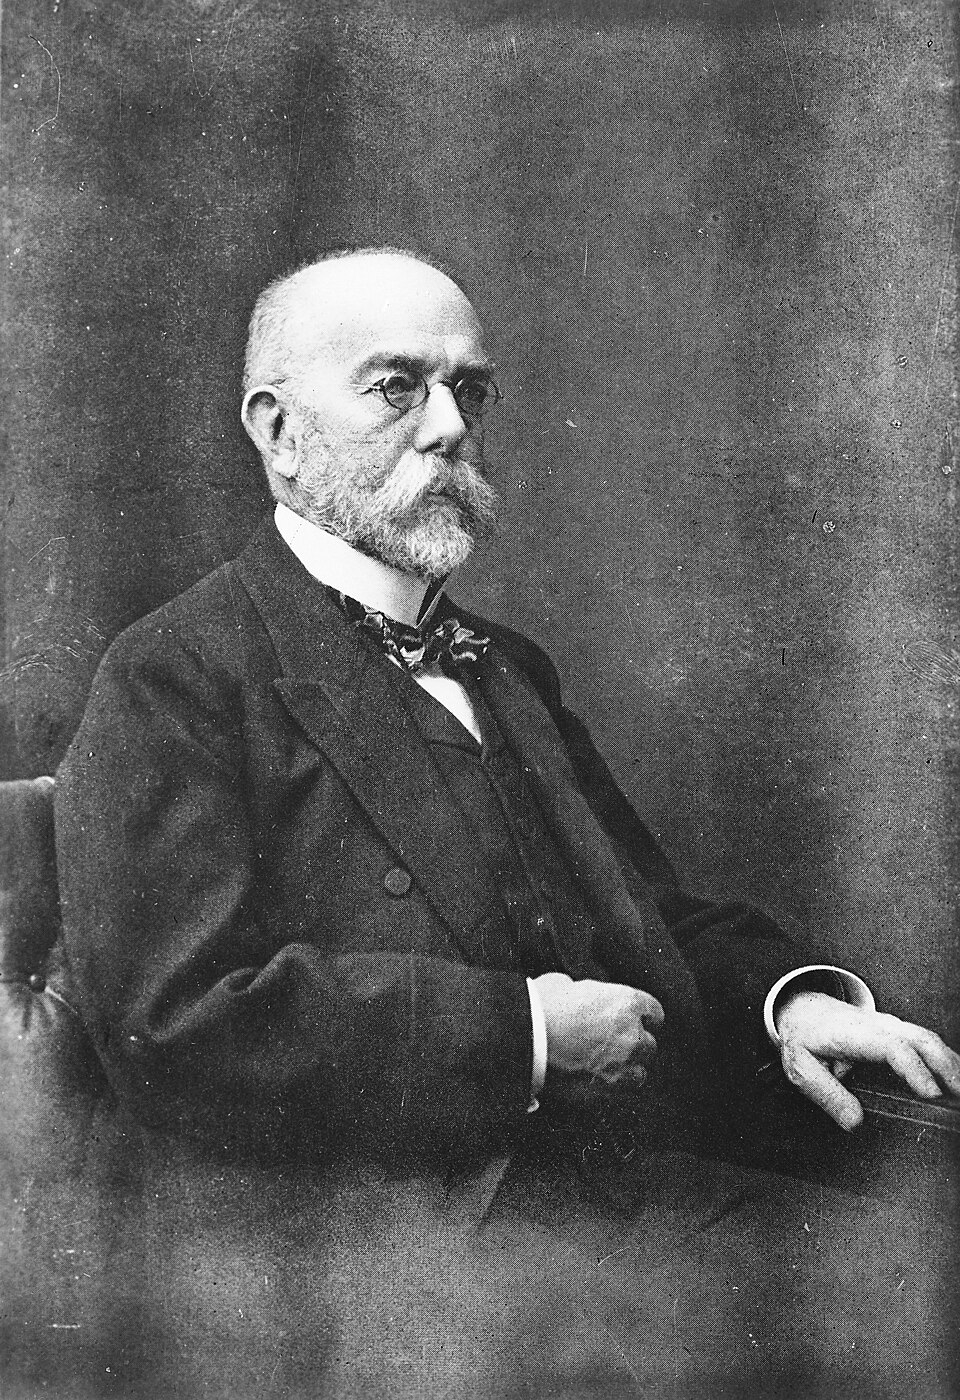
\includegraphics[width=0.30\linewidth]{images/book5/koch.jpg}\hspace{0.04\linewidth}
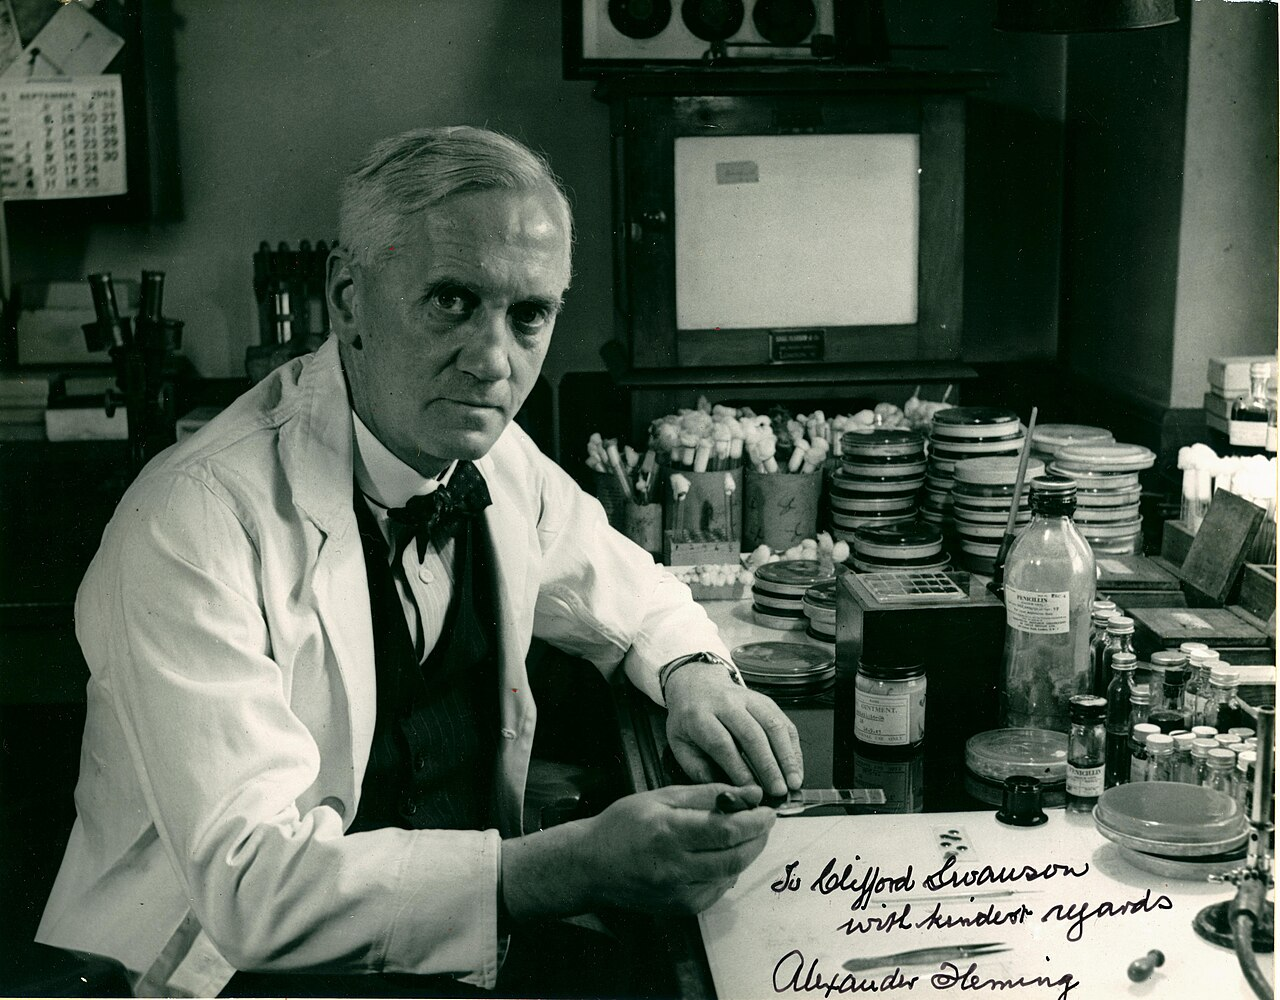
\includegraphics[width=0.56\linewidth]{images/book5/fleming.jpg}

{\small रॉबर्ट कोख, जिन्होंने सिद्ध किया कि विशेष जीवाणु ही विशेष रोग
करते हैं और उन्हें उगाने की विधियाँ बनाईं (वेलकम
संग्रह, CC~BY~4.0)। दाएँ: ऐलेक्ज़ैंडर फ़्लेमिंग अपनी प्रयोगशाला में उस
फफूँद की पट्टिकाओं के साथ जिसका उत्पाद पेनिसिलिन बना (अमेरिकी नौसेना
अभिलेखागार, सार्वजनिक अधिकार)।}
\end{omfigure}

\section{प्रतिजैविक और प्रतिरोध}

\begin{definition}[प्रतिजैविक]\label{def:b3:bacteriology:antibiotics}
\index{प्रतिजैविक}\index{बीटा-लैक्टम}\index{वरणात्मक विषालुता}\index{न्यूनतम निरोधी सांद्रता}
कोई \emph{प्रतिजैविक} ऐसा अणु है जो परपोषी के लिए हानिरहित सांद्रताओं
पर जीवाणुओं को मारता है या उनकी वृद्धि रोक देता है, और वह ऐसे लक्ष्य
पर काम करके ऐसा करता है जो परपोषी के पास नहीं है या भिन्न रूप में है
--- यही \emph{वरणात्मक विषालुता} है। लक्ष्य थोड़े ही हैं। कोशिका-भित्ति:
\emph{$\beta$-लैक्टम} (पेनिसिलिन, सेफ़ैलोस्पोरिन, कार्बापेनेम)
\omterm{def:b3:bacteriology:envelope}{पेप्टिडोग्लाइकन} पेप्टाइड के अंतिम
D-Ala-D-Ala की नकल करते हैं और उन एंज़ाइमों का ऐसिलन कर देते हैं जो उसे
तिर्यक-बद्ध करती हैं, जिससे बढ़ती दीवार कमज़ोर रहती है और कोशिका अपनी ही
स्फीति से फट जाती है; वैनकोमाइसिन स्वयं D-Ala-D-Ala से बँधता है।
राइबोसोम, जिसका जीवाणु रूप सुकेंद्रकी रूप से भिन्न है: ऐमिनोग्लाइकोसाइड
(लघु उपइकाई, जो गलत वाचन कराते हैं), टेट्रासाइक्लिन (tRNA का प्रवेश
रोकते हुए), मैक्रोलाइड और क्लोरैम्फ़ेनिकॉल (बृहत् उपइकाई की निकास-सुरंग
और पेप्टिडिल ट्रांसफ़रेज़)। DNA गाइरेज़ और सांस्थितिकी-एंज़ाइम~IV:
क्विनोलोन। RNA पॉलीमरेज़: रिफ़ैम्पिसिन। फ़ोलेट संश्लेषण, जो प्राणी
नहीं करते: सल्फ़ोनैमाइड और ट्राइमेथोप्रिम। झिल्ली:
पॉलीमिक्सिन, यानी अंतिम उपाय। \emph{न्यूनतम निरोधी सांद्रता}
(MIC) किसी औषध की वह न्यूनतम सांद्रता है जो किसी प्रजाति की दृश्य
वृद्धि रोक देती है; किसी प्रजाति को प्रतिरोधी तब कहते हैं जब उसका MIC
उस सांद्रता से अधिक हो जो औषध रोगी में पाती है।
\end{definition}

\begin{method}[संवेदिता मापना]\label{met:b3:bacteriology:mic}
\index{चक्रिका-विसरण}\index{शोरबा-तनुकरण}
दो परीक्षण। \emph{\omterm{met:b3:bacteriology:mic}{शोरबा-तनुकरण}}: \omterm{def:b3:bacteriology:antibiotics}{प्रतिजैविक} को दोगुने चरणों में रखती
नलिकाओं या कूपों की किसी पंक्ति में कोशिकाओं की कोई नियत संख्या
(प्रति मिलीलीटर लगभग $5\times 10^{5}$) डालिए, रात भर उष्मायित कीजिए, और
पहला स्वच्छ कूप पढ़िए: वही सांद्रता MIC है। \emph{\omterm{met:b3:bacteriology:mic}{चक्रिका-विसरण}}:
प्रजाति को किसी ऐगार पट्टिका पर फैलाइए, कई \omterm{def:b3:bacteriology:antibiotics}{प्रतिजैविकों} की ज्ञात
मात्राओं से भरी कागज़ की चक्रिकाएँ रखिए, उष्मायित कीजिए; औषध बाहर की ओर
विसरित होती है और उसकी सांद्रता दूरी के साथ गिरती है, और वृद्धि उस
त्रिज्या तक रुकी रहती है जहाँ सांद्रता MIC के बराबर हो, इसलिए स्वच्छ
क्षेत्र का व्यास --- अंशांकित सारणियों के सामने पढ़ा जाए तो --- एक ही
पट्टिका पर हर चक्रिका के लिए संवेदिता दे देता है। दोनों परीक्षण एक दिन
लेते हैं; ज्ञात प्रतिरोध-जीनों और उत्परिवर्तनों के लिए जीनोम का
अनुक्रमण उतना ही दिन लेता है और उनकी जगह लेने लगा है।
\end{method}

\begin{definition}[प्रतिरोध]\label{def:b3:bacteriology:resistance}
\index{प्रतिजैविक प्रतिरोध}\index{बीटा-लैक्टमेज़}\index{बहिःस्राव पंप}\index{MRSA}
कोई जीवाणु किसी \omterm{def:b3:bacteriology:antibiotics}{प्रतिजैविक} का प्रतिरोध पाँच में से किसी एक उपाय से
करता है। वह औषध नष्ट कर देता है: \emph{$\beta$-लैक्टमेज़}
$\beta$-लैक्टम वलय का जल-अपघटन करती हैं, और विस्तारित-वर्णक्रम तथा
कार्बापेनेमेज़ रूपांतर अब नवीनतम औषधों को भी नष्ट कर देते हैं। वह
लक्ष्य बदल देता है: किसी राइबोसोमी प्रोटीन या गाइरेज़ में, जिससे औषध
बँधती है, कोई उत्परिवर्तन, या MRSA (मेथिसिलिन-प्रतिरोधी
\emph{Staphylococcus aureus}) में किसी तिर्यक-बंधक एंज़ाइम का कोई अर्जित
जीन जिससे $\beta$-लैक्टम बँधते ही नहीं; वैनकोमाइसिन प्रतिरोध अंतिम
D-Ala की जगह D-लैक्टेट रख देता है, जिसे औषध पहचानती ही नहीं।
वह औषध को \emph{बहिःस्राव पंपों} से बाहर धकेल देता है, जो प्रायः
विशिष्टता में चौड़े होते हैं। वह कोई पोरिन खोकर औषध का भीतर आना रोक देता
है। या वह रुके चरण को किसी वैकल्पिक एंज़ाइम से बाईपास कर देता है।
लक्ष्य-उत्परिवर्तन रोगी में संयोग से प्रति विभाजन $10^{-8}$ से $10^{-6}$
की दरों पर उठते हैं और उपचार के दौरान चुन लिए जाते हैं; एंज़ाइम और पंप
अधिकतर मिट्टी तथा आँत के जीवाणुओं के विशाल भंडार से \omterm{def:b3:genetic-engineering:tools}{प्लाज़्मिडों} पर
अर्जित होते हैं, जिनमें वे युगों तक उन \omterm{def:b3:bacteriology:antibiotics}{प्रतिजैविकों} के विरुद्ध विकसित
हुए जो कवक और दूसरे जीवाणु बनाते हैं। अटल कोशिकाएँ --- वे सुप्त
कोशिकाएँ जो आनुवंशिक रूप से प्रतिरोधी हुए बिना किसी औषध से बच जाती हैं
--- उन पुनरावर्तनों की व्याख्या करती हैं जो ऐसे उपचार के बाद होते हैं
जिसे काम करना चाहिए था।
\end{definition}

\begin{proposition}[प्रतिरोध अनिवार्य क्यों है और उत्तर संयोजन क्यों है]\label{prop:b3:bacteriology:selection}
\index{प्रतिरोध!चयन}\index{संयोजन चिकित्सा!प्रतिजैविक}
$10^{9}$ कोशिकाओं के किसी संक्रमण का उपचार ऐसी औषध से हो जिसके विरुद्ध
प्रतिरोध-उत्परिवर्तन प्रति विभाजन $10^{-8}$ से उठते हों, तो उसमें पहले
से ही लगभग दस प्रतिरोधी कोशिकाएँ हैं; औषध बाकी मार देती है और वे दस
छा जाती हैं --- ठीक \cref{ch:b3:cancer-biology} का अंकगणित, क्योंकि कोई
जीवाणु समष्टि और कोई \omterm{def:b3:cancer-biology:hallmarks}{अर्बुद} दोनों चयन के अंतर्गत विकसित होते क्लोन हैं।
स्वतंत्र लक्ष्यों वाली दो औषधें प्रति विभाजन $10^{-16}$ पर किसी
दोहरे-प्रतिरोधी कोशिका का सामना करती हैं, जो एक अरब कोशिकाओं में नहीं
होती। इसीलिए यक्ष्मा, जिसके घावों में $10^{8}$--$10^{9}$ दंडाणु होते
हैं, 1950 के दशक से एक साथ तीन-चार औषधों से उपचारित की जाती है और इसीलिए
उसकी एक-औषध चिकित्सा ने महीनों में प्रतिरोध पैदा कर दिया था; इसीलिए यह
भी कि \omterm{def:b3:bacteriology:antibiotics}{प्रतिजैविक} का हर उपयोग, चाहे किसी रोगी पर हो या किसी पशु-बाड़े
में, कहीं न कहीं प्रतिरोध चुनता है, और नए \omterm{def:b3:bacteriology:antibiotics}{प्रतिजैविकों} की दर ---
\omterm{def:b3:bacteriology:envelope}{ग्राम-ऋणात्मकों} के विरुद्ध 1960 के दशक से किसी नए वर्ग की एक भी नहीं
--- वही मानदंड है जिसके सामने हानियाँ गिनी जाती हैं। उपाय वही हैं जो
किसी भी विकासात्मक होड़ के हैं: कम काम में लीजिए, संयोजन कीजिए, कोर्स
पूरा कीजिए ताकि अंशतः प्रतिरोधी कोशिकाएँ बचकर न पनपें, और नए लक्ष्य
ढूँढ़िए।
\end{proposition}

\begin{example}[उत्परिवर्ती-चयन खिड़की]\label{ex:b3:bacteriology:window}
किसी प्रजाति का MIC \qty{1}{mg/L} है; उसके प्रथम-चरण प्रतिरोधी
उत्परिवर्ती, जो $10^{7}$ में एक मौजूद हैं, का MIC \qty{8}{mg/L} है।
ऐसी कोई मात्रा जो औषध को \qty{4}{mg/L} पर थामे रखे, वन्य-प्ररूप को मार
देती है और उत्परिवर्तियों को बिना किसी प्रतिस्पर्धा के बढ़ने देती है:
वन्य-प्ररूप के MIC और उत्परिवर्तियों के MIC के बीच की सांद्रता-परास ही
\emph{उत्परिवर्ती-चयन खिड़की} है, और जो उपचार उसमें बैठा रहे वह
प्रतिरोध पनपाता है। \qty{8}{mg/L} से ऊपर की मात्रा दोनों को मार देती है;
बहुत कम मात्रा, या ऐसा कोर्स जो रोगी के अच्छा महसूस करते ही रोक दिया
जाए जब औषध का स्तर खिड़की से होकर गिर रहा हो, इसी तरह कोई प्रतिरोधी
समष्टि बनती है। यही तर्क यक्ष्मा-उपचार की विधियाँ तय करता है: छह
महीने, चार औषधें, और हर एक-चरण उत्परिवर्ती के MIC से ऊपर की मात्राएँ।
\end{example}

\begin{omfigure}
\begin{tikzpicture}
\begin{axis}[
  width=0.7\linewidth, height=5.6cm,
  axis x line=bottom, axis y line=left,
  xmin=0, xmax=24, ymin=0.25, ymax=32, ymode=log,
  xlabel={किसी मात्रा के बाद के घंटे}, ylabel={प्लाज़्मा में औषध (mg/L)},
  xlabel style={font=\small, at={(axis description cs:0.5,-0.12)}, anchor=north}, ylabel style={font=\small},
  tick label style={font=\small}, xtick={0,6,12,18,24}, ytick={0.5,1,2,4,8,16}, yticklabels={0.5,1,2,4,8,16},
  clip=false,
]
\fill[omThm!15] (axis cs:0,1) rectangle (axis cs:24,8);
\addplot[very thick, omDef, domain=0:24, samples=60] {16*exp(-0.15*x)};
\addplot[dashed, gray, domain=0:24, samples=2] {1}; \addplot[dashed, gray, domain=0:24, samples=2] {8};
\node[font=\scriptsize, gray, anchor=south west] at (axis cs:0.3,1.05) {वन्य-प्ररूप का MIC};
\node[font=\scriptsize, gray, anchor=south east] at (axis cs:23.7,8.4) {प्रथम-चरण उत्परिवर्ती का MIC};
\node[font=\scriptsize, omThm!70!black, anchor=west] at (axis cs:13,3.5) {उत्परिवर्ती-चयन खिड़की};
\node[font=\scriptsize, omDef, anchor=south west] at (axis cs:2,13) {किसी मात्रा के बाद प्लाज़्मा स्तर};
\end{axis}
\end{tikzpicture}

{\small उत्परिवर्ती-चयन खिड़की। उत्परिवर्तियों के MIC से ऊपर का
औषध-स्तर सब कुछ मार देता है; दोनों MIC के बीच (छायांकित) वह
वन्य-प्ररूप मारता है और उत्परिवर्ती चुनता है। जिस मात्रा का स्तर घंटों
तक खिड़की से होकर गिरे, या जो कोर्स जल्दी रोक दिया जाए, वह प्रतिरोध पनपाता है।}
\end{omfigure}

\begin{remark}[अधिकांश जीवाणु रोगजनक नहीं हैं]\label{rem:b3:bacteriology:most}
इस अध्याय के चिकित्सालय वाले जीवाणु एक नन्हा अल्पांश हैं। अनुमानित दस
लाख जातियों में से कुछ सौ मानव रोग करती हैं; बाकी नाइट्रोजन, गंधक और
कार्बन के चक्र चलाती हैं (वर्ष~2 का खंड), हर शिंब की नाइट्रोजन स्थिर
करती हैं, हर रोमंथी में सेलुलोज़ पचाती हैं, और
\cref{ch:b3:microbiomes} के सूक्ष्मजीवियों को बनाती हैं, जिनका
\omterm{def:b3:bacteriology:antibiotics}{प्रतिजैविक} उपचार में ह्रास हर कोर्स की एक लागत है। स्वयं \omterm{def:b3:bacteriology:antibiotics}{प्रतिजैविक}
उन्हीं के अणु हैं --- अस्पतालों के होने से बहुत पहले मिट्टी के
जीवाणुओं और कवकों के बीच विकसित हुए हथियार और संकेत --- और अधिकांश
प्रतिरोध-जीन भी।
\end{remark}

\section{अभ्यास}

\begin{exercise}[$\star$]\label{exo:b3:bacteriology:1}
\omterm{def:b3:bacteriology:envelope}{ग्राम-धनात्मक} और \omterm{def:b3:bacteriology:envelope}{ग्राम-ऋणात्मक} आवरणों का वर्णन कीजिए और समझाइए कि
\omterm{met:b3:bacteriology:gram}{ग्राम अभिरंजन} उनमें भेद कैसे करता है।
\end{exercise}

\begin{exercise}[$\star$]\label{exo:b3:bacteriology:2}
प्रति मिलीलीटर $10^{3}$ कोशिकाओं का कोई संवर्धन चरघातांकी वृद्धि के
\qty{8}{h} में $10^{9}$ तक पहुँचता है। पीढ़ियों की संख्या, पीढ़ी-काल और
$\mu$ ढूँढ़िए।
\end{exercise}

\begin{exercise}[$\star$]\label{exo:b3:bacteriology:3}
क्षैतिज जीन-स्थानांतरण के तीन मार्गों के नाम दीजिए और हर एक को दिखाने
वाला शास्त्रीय प्रयोग बताइए।
\end{exercise}

\begin{exercise}[$\star$]\label{exo:b3:bacteriology:4}
पेनिसिलिन, स्ट्रेप्टोमाइसिन, सिप्रोफ़्लोक्सैसिन और रिफ़ैम्पिसिन का
लक्ष्य दीजिए, और बताइए कि हर एक वरणात्मक रूप से विषालु क्यों है।
\end{exercise}

\begin{exercise}[$\star\star$]\label{exo:b3:bacteriology:5}
किसी केमोस्टैट में $\mu_{\max} = \qty{0.8}{h^{-1}}$, $K_{S} =
\qty{0.02}{g/L}$, $S_{0} = \qty{2}{g/L}$, $Y = 0.4$ हैं। $S^{*}$ तथा
$X^{*}$ निकालिए, $D = 0.2$,
$0.6$ और $0.79$ h$^{-1}$ पर, और वह \omterm{thm:b3:bacteriology:monod}{तनुकरण दर} भी जिस पर बहना शुरू होता है।
\end{exercise}

\begin{exercise}[$\star\star$]\label{exo:b3:bacteriology:6}
\cref{prop:b3:bacteriology:threshold} का उपयोग करते हुए किसी स्क्विड के
प्रकाश-अंग ($k =
\qty{0.01}{h^{-1}}$) और बहते समुद्री जल ($k = \qty{10}{h^{-1}}$) में
\omterm{def:b3:bacteriology:quorum}{गणपूर्ति संवेदन} की देहली-घनत्व की तुलना कीजिए, जहाँ $p = 100$ अणु प्रति
कोशिका प्रति घंटा और $A_{\text{देहली}} =
\qty{10}{nmol/L}$ ($6\times 10^{12}$ अणु प्रति लीटर) हो।
\end{exercise}

\begin{exercise}[$\star\star$]\label{exo:b3:bacteriology:7}
किसी \omterm{met:b3:bacteriology:mic}{चक्रिका-विसरण} पट्टिका पर तीन औषधों के लिए $25$, $12$ और
\qty{0}{mm} के क्षेत्र दिखते हैं। हर एक की व्याख्या कीजिए, और समझाइए कि
किसी क्षेत्र-व्यास को किसी MIC में क्यों बदला जा सकता है।
\end{exercise}

\begin{exercise}[$\star\star$]\label{exo:b3:bacteriology:8}
समझाइए कि कोई एक \omterm{def:b3:bacteriology:hgt}{संयुग्मन} घटना किसी संवेदी \emph{Klebsiella} को पाँच
\omterm{def:b3:bacteriology:antibiotics}{प्रतिजैविकों} के प्रति प्रतिरोधी कैसे बना सकती है, और प्रतिरोध-जीन इतनी
बार \omterm{def:b3:genetic-engineering:tools}{प्लाज़्मिडों} पर साथ-साथ क्यों मिलते हैं।
\end{exercise}

\begin{exercise}[$\star\star$]\label{exo:b3:bacteriology:9}
किसी रोगी में $10^{9}$ जीवाणु हैं और वह ऐसी औषध लेता है जिसके विरुद्ध
प्रतिरोध प्रति विभाजन $10^{-7}$ से उठता है। आरंभ पर प्रत्याशित
प्रतिरोधी कोशिकाएँ निकालिए; फिर दो स्वतंत्र औषधों के साथ। अटल कोशिकाएँ
एक भिन्न समस्या क्यों हैं?
\end{exercise}

\begin{exercise}[$\star\star\star$]\label{exo:b3:bacteriology:10}
दिखाइए कि केमोस्टैट की स्थायी अवस्था स्थिर है: $X$ को $X^{*}$ से
थोड़ा ऊपर विक्षुब्ध कीजिए और $\mathrm{d}S/\mathrm{d}t$ तथा
$\mathrm{d}X/\mathrm{d}t$ के चिह्नों का पीछा कीजिए। फिर समझाइए कि किसी
केमोस्टैट में एक ही पोषक के लिए प्रतिस्पर्धा करती दो जातियाँ स्थायी
अवस्था पर सह-अस्तित्व क्यों नहीं रख सकतीं, और किसी दिए हुए $D$ पर कौन जीतती है।
\end{exercise}

\begin{exercise}[$\star\star\star$]\label{exo:b3:bacteriology:11}
\omterm{def:b3:bacteriology:quorum}{स्वप्रेरक} अपनी ही सिंथेज़ प्रेरित करता है।
\cref{prop:b3:bacteriology:threshold} का प्रतिरूप ऐसे बदलिए कि $p$
$p_{0}$ से उछलकर
$p_{1} \gg p_{0}$ हो जाए जब $A > A_{\text{देहली}}$ हो, और दिखाइए कि तंत्र की घनत्वों की किसी परास पर
दो स्थिर अवस्थाएँ हो सकती हैं (शैथिल्य): जो समष्टि चालू हो चुकी हो वह
उस घनत्व पर भी चालू रहती है जिस पर कोई अनजान समष्टि बंद रहती। इसका
जैविक उपयोग क्या है?
\end{exercise}

\begin{exercise}[$\star\star\star$]\label{exo:b3:bacteriology:12}
उत्परिवर्ती-चयन खिड़की समझाइए और उससे इनमें से हर एक के पक्ष या विपक्ष
में तर्क दीजिए: (क) छोटे कोर्स में ऊँची मात्राएँ; (ख) लंबे कोर्स में
कम मात्राएँ; (ग) लक्षण मिटते ही रोक देना; (घ) \omterm{thm:b3:cancer-biology:goldie-coldman}{संयोजन चिकित्सा}।
\end{exercise}

\section{समस्या: एक केमोस्टैट और एक चिकित्सालय}

\begin{problem}[{सप्तांत समस्या --- कोई संवर्धन किसी फ्लास्क में उगाया
और किसी केमोस्टैट में थामा गया, कोई ज्योतिर्मय जीवाणु अपनी गणपूर्ति तक
गिना गया, और कोई संक्रमण प्रतिरोध के अंकगणित के सामने उपचारित किया गया,
जिसका अंत केमोस्टैट की कोशिकाओं, उस घनत्व जिस पर प्रकाश चालू होता है,
और इस संभावना पर होता है कि कोई दो-औषध कोर्स किसी प्रतिरोधी कोशिका से
मिले}]
\label{pb:b3:bacteriology:1}
आँकड़े: \qty{37}{\celsius} पर \emph{E.~coli}, $T = \qty{20}{min}$; एक
कोशिका का भार \qty{1}{pg}। केमोस्टैट: $V = \qty{1}{L}$, $F = \qty{0.5}{L/h}$,
$\mu_{\max} = \qty{1.0}{h^{-1}}$, $K_{S} = \qty{0.01}{g/L}$, $S_{0} =
\qty{2}{g/L}$ ग्लूकोज़, $Y = 0.5$। \emph{Vibrio}: $p = 500$ \omterm{def:b3:bacteriology:quorum}{स्वप्रेरक}
अणु प्रति कोशिका प्रति घंटा, $A_{\text{देहली}} = 6\times 10^{12}$
अणु प्रति लीटर (\qty{10}{nmol/L}), प्रकाश-अंग में $k = \qty{0.05}{h^{-1}}$।
संक्रमण: $10^{9}$ कोशिकाएँ; औषध A के प्रति प्रतिरोध
प्रति विभाजन $10^{-8}$, औषध B के प्रति $10^{-7}$; A का वन्य-प्ररूप MIC
\qty{1}{mg/L}, प्रथम-चरण उत्परिवर्ती \qty{8}{mg/L}; कोई मात्रा
\qty{16}{mg/L} देती है जो \qty{4}{h} के अर्ध-आयु काल से गिरती है।

\medskip
\noindent\textbf{भाग I --- फ्लास्क।}
\begin{enumerate}
  \item \qty{100}{mL} शोरबे में एक कोशिका। चरघातांकी वृद्धि के
        \qty{6}{h} बाद कितनी कोशिकाएँ, और प्रति mL कितना घनत्व?
  \item शोरबा अधिक-से-अधिक प्रति mL $2\times 10^{9}$ कोशिकाएँ पाल सकता
        है। वृद्धि कब रुकती है, और संवर्धन की कोशिकाओं का द्रव्यमान
        क्या है?
  \item एक कोशिका के वंशजों को पृथ्वी के द्रव्यमान ($6\times 10^{27}$ g)
        तक पहुँचने में कितना समय लगेगा? टिप्पणी कीजिए।
  \item \omterm{def:b3:bacteriology:phases}{स्थिर प्रावस्था} की कोशिकाएँ ताज़ा माध्यम में डालने पर \omterm{def:b3:bacteriology:phases}{विलंब
        प्रावस्था} \qty{1}{h} रहती है, और चरघातांकी कोशिकाएँ लेने पर
        लगभग कुछ नहीं। समझाइए।
  \item $\mu$ निकालिए, $T$ से। यदि माध्यम ऐसी शर्करा पर बदला जाए जिस पर
        $T = \qty{60}{min}$ हो, तो $\mu$ क्या है, और \qty{6}{h} बाद
        कोशिकाओं की संख्या किस गुणक से गिर जाती है?
  \item स्थिर संवर्धन का कोई प्रतिदर्श किसी पट्टिका पर फैलाया जाता है
        और $200$ बस्तियाँ देता है, किसी $10^{-6}$ तनुकरण के
        \qty{0.1}{mL} से।
        जीवक्षम गणना क्या है, और वह किसी सूक्ष्मदर्शी गणना से भिन्न
        क्यों हो सकती है?
\end{enumerate}

\medskip
\noindent\textbf{भाग II --- केमोस्टैट।}
\begin{enumerate}[resume]
  \item \omterm{thm:b3:bacteriology:monod}{तनुकरण दर} $D$ और वह पीढ़ी-काल निकालिए जो संवर्धन को अपनाना
        पड़ता है।
  \item $S^{*}$ और $X^{*}$ निकालिए (g/L में और प्रति mL कोशिकाओं में)।
  \item प्रति घंटा कितनी कोशिकाएँ पात्र से निकलती हैं? संवर्धन एक महीने
        में कितनी पीढ़ियाँ पार करता है?
  \item पंप बढ़ाकर $F = \qty{0.95}{L/h}$ कर दिया जाता है। नए $S^{*}$ और
        $X^{*}$? $F = \qty{1.1}{L/h}$ पर क्या होता है?
  \item कोई उत्परिवर्ती प्रकट होता है जिसका $\mu_{\max} = \qty{1.2}{h^{-1}}$
        है और $K_{S}$ वही। $D = 0.5$ पर उसे कौन-सा $S^{*}$ चाहिए, और
        मूल प्रजाति का क्या होता है? (\cref{exo:b3:bacteriology:10} का
        उपयोग कीजिए।)
  \item एक महीने की बारी $700$ पीढ़ियाँ है। यदि कोई लाभकारी उत्परिवर्तन
        प्रति विभाजन $10^{-9}$ से उठे और पात्र में $10^{12}$
        कोशिकाएँ हों, तो प्रति पीढ़ी कितने लाभकारी उत्परिवर्तन उठते
        हैं? इससे किसी केमोस्टैट में विकास के बारे में क्या निकलता है?
\end{enumerate}

\medskip
\noindent\textbf{भाग III --- गणपूर्ति।}
\begin{enumerate}[resume]
  \item प्रकाश-अंग में प्रकाश की देहली कोशिका-घनत्व प्रति mL कोशिकाओं
        में निकालिए।
  \item प्रकाश-अंग में \qty{1}{\micro L} जीवाणु प्रति mL $10^{10}$ पर
        रहते हैं। \omterm{def:b3:bacteriology:quorum}{स्वप्रेरक} देहली से किस गुणक ऊपर है?
  \item समुद्री जल में संकेत $k = \qty{20}{h^{-1}}$ से बह जाता है।
        देहली-घनत्व? खुले समुद्र की प्रति mL $10^{2}$ कोशिकाओं से तुलना
        कीजिए।
  \item भोर में स्क्विड द्वारा \qty{90}{\%} जीवाणु निकाल देने के बाद,
        बचे प्रति mL $10^{9}$ को, हर \qty{2}{h} में विभाजित होते हुए,
        प्रति mL $10^{10}$ फिर बनाने में कितना समय लगेगा? बीच में क्या
        प्रकाश बुझ जाता है?
  \item हर चमकती कोशिका अपनी ऊर्जा का लगभग \qty{20}{\%} प्रकाश पर
        खर्च करती है। समुद्र में कोई अँधेरी कोशिका वरीय क्यों है, और
        अंग में क्यों नहीं?
  \item कोई रोगजनक इसी तंत्र से अपने विष तब तक टालता है जब तक वह
        संख्या में न हो जाए। ऐसी कोई औषध-रणनीति सुझाइए जो इसका लाभ
        उठाए और बताइए कि वह किसी \omterm{def:b3:bacteriology:antibiotics}{प्रतिजैविक} से धीरे प्रतिरोध क्यों चुन
        सकती है।
\end{enumerate}

\medskip
\noindent\textbf{भाग IV --- चिकित्सालय।}
\begin{enumerate}[resume]
  \item उपचार के आरंभ पर A के प्रति प्रतिरोधी कोशिकाओं की प्रत्याशित
        संख्या; B के प्रति; दोनों के प्रति।
  \item इसकी प्रायिकता कि A के प्रति प्रतिरोधी कोई कोशिका न हो; दोनों
        के प्रति न हो।
  \item मात्रा के बाद औषध-स्तर \qty{8}{mg/L} तक कब गिरता है, और
        \qty{1}{mg/L} तक? प्रति मात्रा वह कितनी देर उत्परिवर्ती-चयन
        खिड़की में बिताता है?
  \item यदि औषध हर \qty{12}{h} में दी जाए, तो समय का कितना अंश स्तर
        खिड़की में रहता है, और अकेली A के दस दिन के कोर्स पर इससे
        क्या पूर्वानुमान निकलता है?
  \item ऐसा कोई मात्रा-परिवर्तन सुझाइए जो स्तर को पूरे समय
        \qty{8}{mg/L} से ऊपर रखे (आवश्यक अंतराल या मात्रा निकालिए), और
        उसकी लागत बताइए।
  \item $10^{4}$ में एक कोशिका कोई अटल कोशिका है, जो सुप्त है और दोनों
        में से किसी औषध की किसी भी सांद्रता से अछूती। कोर्स से कितनी
        बचती हैं, औषध हटते ही क्या होता है, और उपचार की लंबाई के लिए
        इसका क्या अर्थ है?
  \item सारांश दीजिए: केमोस्टैट में प्रति mL कोशिकाएँ (प्रश्न~8),
        प्रकाश की देहली-घनत्व (प्रश्न~13), और इसकी प्रायिकता कि
        दो-औषध कोर्स को कोई प्रतिरोधी कोशिका न मिले (प्रश्न~20)।
\end{enumerate}
\end{problem}
